\documentclass[twocolumn]{ctexart}
\CTEXsetup[format={\Large\bfseries}]{section}%让section指令左对齐
\renewcommand{\abstractname}{}%去掉摘要头上的标题
\newcommand{\upcite}[1]{\textsuperscript{\textsuperscript{\cite{#1}}}}%右上角引用文献的命令
\usepackage[margin=1.85cm]{geometry}%调整页边距
\usepackage{pifont}%提供圆圈数字输入
\usepackage{graphicx}%插入图片
\usepackage{authblk}%作者、单位
\usepackage{amsmath, bm}%数学公式宏包
\usepackage{esint}%使重积分符号更加紧凑,必须加在amsmath后
\usepackage{amssymb}%特殊数学符号
\usepackage{caption}%图片标题处理
\usepackage{float}%处理图表浮动插入
\usepackage[section]{placeins}%防止图表浮动跨过section
\usepackage{subfigure}%插入多图时用子图显示的宏包
\pagestyle{plain}%页码
\setCJKfamilyfont{zhsong}[AutoFakeBold = {2.17}]{SimSun}
\setCJKmainfont{SimSun}[BoldFont=FandolSong-Bold]
\renewcommand*{\songti}{\CJKfamily{zhsong}}%定义新宋体命令
\setlength{\belowcaptionskip}{-2pt}
\begin{document}
	
	\zihao{5}%设置全文字号为五号
	\everymath{\displaystyle}%设置所有数学公式为displaystyle形式
	\abovedisplayshortskip=5pt%设置数学公式间距
	\belowdisplayshortskip=5pt
	\abovedisplayskip=5pt
	\belowdisplayskip=5pt
	\lineskiplimit=4pt
	\lineskip=4pt
	\title{\vspace{-2cm}{\heiti {\zihao{2}人工智能安全挑战:对抗攻击}} }%标题
	\date{}%不显示日期
	\author[1]{\zihao{-4}任威 \vspace{-1.5em}}%作者名称
	\affil[1]{\vspace{-6em}{{\zihao{6}{\kaishu 广州大学}}}}%作者单位
	\twocolumn[
	\begin{@twocolumnfalse}
		\maketitle 
		\begin{abstract}
			\newgeometry{left=1.5cm, right=1.5cm}%调整摘要部分的页边距,与正文对齐
			\noindent{\zihao{-5}{\heiti 摘~~~要 }{\kaishu ~~~随着深度学习在各个领域的广泛应用,对抗攻击对于模型的安全性构成了严峻挑战。本文深入探讨了对抗攻击的分类及其不同类型的特点,包括白箱攻击、黑箱攻击,以及基于评分、梯度和决策的攻击方法。对抗防御技术也得到了关注,探讨了对抗训练、模型调整、对抗样本检测和随机性增强等多种防御方法。特别关注了最新的方差调整方法,以提高基于梯度攻击的效果和可转移性。}}\\
			\noindent{\zihao{-5}\heiti 关键词 }~~~{\zihao{-5}\kaishu 对抗攻击,人工智能安全,深度学习}\\
			\\
		\end{abstract}
	\end{@twocolumnfalse}
	]%双栏环境下单栏的摘要
	
	\section{{\zihao{4}{\songti 引言}}\vspace{-0.4em}}
%	\subsection{{\songti 第一小节}\vspace{-0.6em}}
	近年来,机器学习取得了长足的进步,尤其是深度学习在各个领域的广泛应用。深度学习作为机器学习的重要分支,在计算机视觉、自然语言处理、语音识别、恶意软件检测、分类问题、生物科学等领域都取得了成功。特别是在计算机视觉方面,它在自动驾驶、智能工业机器和移动应用等领域有着重要的应用前景。
	
	然而,深度神经网络模型容易受到对抗攻击,这种攻击利用微小且人眼无法察觉的扰动,导致模型错误分类输入样本。这些对抗样本不仅可用于图像分类,还可应用于现实场景,比如干扰交通标志识别系统或自动驾驶车辆。
	
	尽管深度学习在多个领域得到应用,但其安全性问题限制了在安全关键领域的应用。为了解决这一挑战,对抗攻击领域已提出了多种生成对抗样本的方法,包括增强攻击强度、改进模型迁移和优化计算能力等途径。
%	\subsection{{\songti 第二小节}\vspace{-0.6em}}
%	这是一段数学公式
%	\begin{equation}
%		\begin{aligned}
%			p=\frac{L^{2}}{G M m^{2}}, \quad \varepsilon=\sqrt{1+\frac{2 E L^{2}}{G^{2} M^{2} m^{3}}} \\
%		\end{aligned}\tag{1.2.1}
%	\end{equation}
%	\begin{equation}
%		\begin{aligned}
%			\mathrm{~d} \theta=\frac{\mathrm{d} r / r^{2}}{\sqrt{\left(\dfrac{\varepsilon}{p}\right)^{2}-\left(\dfrac{1}{r}-\dfrac{1}{p}\right)^{2}}} .
%		\end{aligned}\tag{1.2.2}
%	\end{equation}
	\section{{\zihao{4}{\songti 相关概念}}\vspace{-0.6em}}
	\subsection{{\songti 对抗攻击概念}\vspace{-0.6em}}
	对抗学习是一种基于博弈论的人工智能学习方法,涉及两个或多个智能体之间的相互对抗。每个智能体都试图通过欺骗或干扰对方来提高自身的性能。例如,在网络安全领域,可以利用对抗学习来训练入侵检测系统,使其能够更好地识别和防范网络攻击;在金融交易领域,可以运用对抗学习来提高风险评估和欺诈检测的准确性。
	近年来,随着机器学习的快速发展与广泛应用,对抗学习这一领域得到了前所未有的蓬勃发展。然而,随着AI的发展,对抗技术也在不断演进,引发了广泛关注。因此,我们需要更深入地理解其原理,并寻找有效的防御策略。
	
	\subsection{{\songti 生成对抗网络}\vspace{-0.6em}}
	生成对抗网络(GAN)是一种对抗学习的重要技术。如图1所示,它由两个主要组件组成:生成器和判别器。生成器旨在创造逼真的图像或数据,而判别器则试图将生成器产生的数据与真实数据区分开来。这两个部分相互博弈,通过对抗训练,使得生成器逐渐学会生成与真实数据难以区分的合成数据。
	\begin{figure}[htbp]
		\centering
		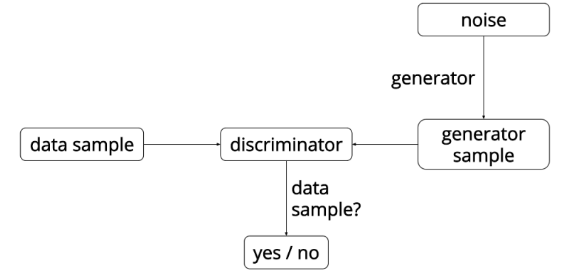
\includegraphics[width=0.5\textwidth]{fig1.png}
		\caption{GAN网络整体结构.}
		\label{fig}
	\end{figure}
	
	在GAN中,生成器通过学习真实数据的分布模式来生成新的数据样本,而判别器则努力区分生成的样本与真实数据。这种对抗过程持续迭代训练,使得生成器能够逐渐提高生成数据的逼真度,直至达到与真实数据相媲美的程度。
	
	GAN的应用十分广泛,不仅局限于图像生成领域,还涉及音频合成、自然语言处理等多个领域。其独特的对抗学习机制使得其在生成高质量数据方面具有显著优势,为模仿、合成和生成各种类型的数据提供了强大的工具。
	
	\subsection{{\songti 对抗样本}\vspace{-0.6em}}
	对抗样本是指对机器学习模型具有误导性的输入,通过对原始输入进行微小的、人类难以察觉的变化,使模型产生错误的输出。这种输入的变化可以是对图像、文本、声音等数据进行微小扰动,足以使模型做出错误的推断或分类。如图 2 所示,原有的自然样本来源于ImageNet, 识别模型为GoogLeNet, 通过在熊猫图片中添加肉眼不可见的微小扰动, 使模型的识别结果变为了“长臂猿”.
	\begin{figure}[htbp]
		\centering
		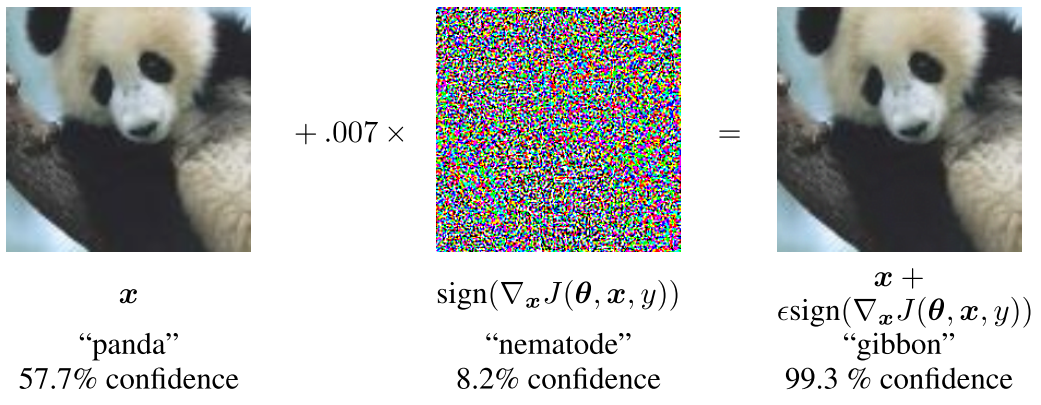
\includegraphics[width=0.5\textwidth]{fig2.png}
		\caption{对抗样本.}
		\label{fig}
	\end{figure}
	
	对抗样本的存在对机器学习模型的安全性构成挑战,因为它们可能导致模型做出不可预测或错误的预测,即使这些变化对人类观察者来说是不可见的。这种现象引发了对模型的鲁棒性和可靠性的担忧,尤其是在安全关键领域,如自动驾驶、医疗诊断和安全检测等应用中。
	
	\subsection{{\songti 对抗防御}\vspace{-0.6em}}
	对抗防御是指针对对抗攻击和对抗样本的一系列防御措施和技术。在机器学习和深度学习中,对抗防御旨在提高模型的鲁棒性,使其更能抵抗对抗攻击,防止模型在面对对抗性样本时产生误判或误分类。
	
	对抗防御的方法多种多样,其中一些主要方法包括:
	
	\pmb{1. 对抗训练}\textbf{(Adversarial Training):}这种方法通过在训练过程中故意添加对抗样本,使模型更好地学习对抗性特征,并提高其对对抗攻击的抵抗能力。
	
	\pmb{2. 防御性调整模型}\textbf{(Defensive Model Adjustments):}这类方法包括调整模型的结构或参数,使其更具鲁棒性,例如增加正则化项、降低模型的复杂度或者改进模型的架构。
	
	\pmb{3. 对抗样本检测和过滤}\textbf{(Adversarial Sample Detection and Filtering):}该方法旨在识别和过滤出对抗性样本,以防止它们影响模型的决策。
	
	\pmb{4. 随机性增强}\textbf{(Randomization Techniques):} 通过引入随机性扰动或噪声,使模型更难以受到对抗攻击。
	
	\pmb{5. 生成对抗网络(GAN)防御方法:} 利用生成对抗网络(GAN)来生成对抗样本,以便训练模型更好地抵御这些对抗样本的影响。
	
	这些防御措施并非完全消除对抗攻击的可能性,而是试图提高模型对对抗性样本的鲁棒性。对抗防御是一个活跃的研究领域,不断涌现新的方法来提高机器学习模型对对抗攻击的抵御能力。
	
	\section{{\zihao{4}{\songti 对抗攻击分类}}\vspace{-0.6em}}
	
	\subsection{{\songti 白盒攻击}\vspace{-0.6em}}
	白箱攻击中,攻击者具有对目标模型的全部信息,包括模型的训练数据、类型、结构和参数等。这种情况下,攻击者可以充分了解目标模型的内部机制,利用这些信息来生成对抗样本。尽管这种情况假设了攻击者具有极高的能力,但可以用于评估模型安全性的下限,且与“基于迁移的攻击”结合可以产生有意义的研究成果。
	
	\subsubsection{{\songti 基于梯度的攻击}\vspace{-0.6em}}
	这类攻击利用输入样本的梯度信息,通过观察目标模型对输入样本的输出梯度,然后在输入空间中搜索最有效的对抗样本。尽管攻击者无法直接访问目标模型的参数,但通过模型输出对输入样本的梯度计算,攻击者能够生成能够迷惑模型的对抗样本。这种攻击方法不需要目标模型的具体信息,仅需通过输入输出信息来构建对抗样本。
	
	2021年,Wang和He提出了一项名为"方差调整"(variance tuning)的新方法[10],旨在增强基于迭代梯度的攻击方法的效果,并提高其攻击的可转移性。该方法通过考虑梯度在每次迭代中的变化,而不是直接使用动量累积的梯度,来进一步调整当前梯度方向。这种方法旨在使更新方向更加不稳定,以避免陷入局部最优点。其关键思想是减少每次迭代时的梯度变化,以稳定更新方向,并在搜索过程中摆脱局部最优解。作者首先定义了梯度变化,即:
	\begin{equation*}
		V_{\epsilon^{\prime}}^{g}(x)=\mathbb{E}_{\|x^{\prime}-x\|_{p}<\epsilon^{\prime}}\left[\nabla_{x^{\prime}}J\left(x^{\prime},y;\theta\right)\right]-\nabla_{x}J(x,y;\theta) \tag{1}
	\end{equation*}
	
	其中,${\epsilon^{\prime}} = \beta \times \epsilon $,其中$\beta$为超参数,$\epsilon$表示扰动的上界。由于输入空间的连续性,难以直接获得前一项的值,因此可以通过对$N$个样本进行采样来近似计算。
	\begin{equation*}
		V(x)=\dfrac{1}{N}\sum_{i=1}^{N}\nabla_{x^i}J\left(x^i,y;\theta\right)-\nabla_xJ(x,y;\theta) \tag{2}
	\end{equation*}
	
	其中,$x_i = x + r_i$,其中$ r_i$ 符合均匀分布 $U[-\beta \cdot \epsilon^d, \beta \cdot \epsilon^d]$。在实现过程中,即对 $x$进行多次随机扰动后取平均值,然后计算变化。
	\subsection{{\songti 黑盒攻击}\vspace{-0.6em}}
	2017年,Papernot等研究人员在[8]中首次提出了一种基于黑盒攻击的方法。该方法通过生成替代模型来近似攻击目标模型的决策边界,并利用这个替代模型生成对抗样本,最终用这些对抗样本来攻击原始目标模型。在训练过程中,他们有效地利用雅可比矩阵来获取查询结果,从而减少了对目标模型的查询次数。由于该方法不依赖梯度信息,传统的梯度掩码防御策略对这种攻击方法失效。
	
	在黑箱攻击中,攻击者不知道目标模型的内部细节,只能观察其对输入样本的输出结果。已有的黑箱攻击大致分为三类:
	\subsubsection{{\songti 基于迁移的攻击}\vspace{-0.6em}}
	这类攻击利用迁移现象:针对某一机器学习模型的对抗样本也可能欺骗其他模型。攻击者首先训练一个与目标模型相似的替代模型,再使用白箱攻击算法生成能欺骗替代模型的对抗样本。根据迁移现象,这些对抗样本大概率也能欺骗攻击者真正想要攻击的目标模型。
	一般来说,传统的域适应问题一般会选用固定的特征 (fixed feature represenatations),但是[6]提出的对抗迁移网络则关注于如何在不同域之间选择可供迁移的特征(transferable features)。域对抗迁移网络(DANN),如图3所示:
	\begin{figure}[htbp]
		\centering
		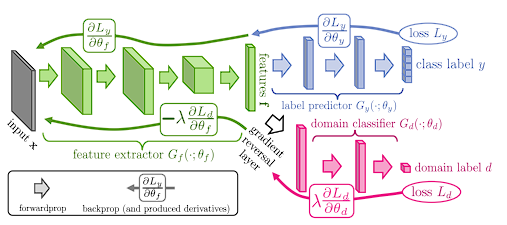
\includegraphics[width=0.5\textwidth]{fig3.png}
		\caption{DANN结构.}
		\label{fig}
	\end{figure}
	
	图示蓝色部分为abel predictor,对来自源域的数据进行分类,尽可能分出正确的标签。
	
	图示红色部分为域判别器(domain classifier),对特征空间的数据进行分类,尽可能分出数据来自哪个域。
	
	其中,特征提取器和标签分类器构成了一个前馈神经网络。然后,在特征提取器后面,加上一个域判别器,中间通过一个梯度反转层 (gradient reversal layer, GRL) 连接。在训练的过程中,对来自源域的带标签数据,网络不断最小化标签预测器的损失 (loss)。对来自源域和目标域的全部数据,网络不断最小化域判别器的损失。
	
	\subsubsection{{\songti 基于评分的攻击}\vspace{-0.6em}}
	这种攻击根据目标模型对输入样本属于各个类别的概率评分,估计模型损失函数的梯度,进而生成对应的对抗样本。整个过程不需要目标模型的内部信息或额外训练替代模型。
	
	基于零阶优化(ZOO)的攻击来直接估计目标DNN的梯度在[3]中被提出,以生成对抗性示例。使用零阶随机坐标下降以及降维、分层攻击和重要性抽样技术来有效地攻击黑盒模型。通过利用零阶优化,可以实现对目标DNN的改进攻击,从而无需训练替代模型,避免攻击可转移性的损失。
	
	首先对输入 $x $ 进行一个扰动 $x = x + h $,其中 $h = 0.0001 $是一个常量值,$e$ 是一个标准单位向量。最后使用对称差商(symmetric difference quotient )来估计梯度
	\begin{equation*}
		\hat{g}_i:=\frac{\partial f(\mathbf{x})}{\partial\mathbf{x}_i}\approx\frac{f\left(\mathbf{x}+h\mathbf{e}_i\right)-f\left(\mathbf{x}-h\mathbf{e}_i\right)}{2h} \tag{3}
	\end{equation*}
	
	在增加一次查询就能得到二阶信息
	\begin{equation*}
		\hat{h}_i:=\frac{\partial^2f(\mathbf{x})}{\partial\mathbf{x}_{ii}^2}\approx\frac{f\left(\mathbf{x}+h\mathbf{e}_i\right)-2f(\mathbf{x})+f\left(\mathbf{x}-h\mathbf{e}_i\right)}{h^2} \tag{4}
	\end{equation*}
	
	有了这两个梯度估计值,就可以直接对 $x$ 进行梯度下降优化。
	\subsubsection{{\songti 基于决策的攻击}\vspace{-0.6em}}
	这类攻击仅依靠目标模型对每个输入样本的最终分类决策来生成对抗样本。相较前两类,这种攻击方法不需要训练替代模型或获取每个样本的概率评分,但通常需要更多次向目标模型查询以达到最佳攻击性能。
	
	在[2]中针对decision-based攻击提出了Boundary Attack。 $\tilde{o}$ 是对抗样本,$\tilde{o}^k$ 代表第 $k$ 迭代的对抗样本。该算法从一个已经是对抗样本的点初始化,然后沿着对抗性和非对抗性区域之间的边界执行随机游走,这样它留在对抗性区域和到目标图像的距离降低了。算法主要的超参数是扰动总长度 $\delta$ 和到原图距离的步长 $ \epsilon $ 。如图4所示,所谓正交扰动,就是先水平动一下,然后垂直靠近边界,动态调整参数。
	
	\begin{figure}[htbp]
		\centering
		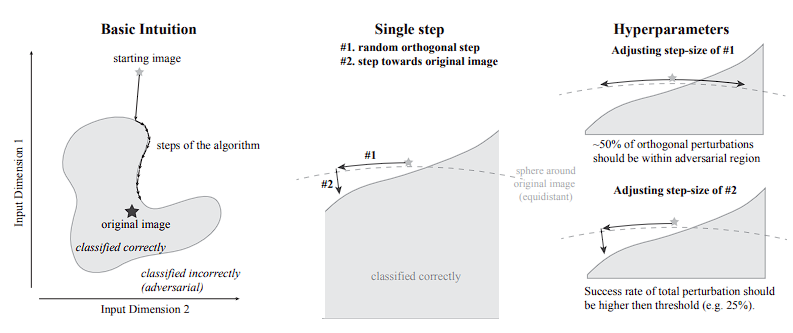
\includegraphics[width=0.5\textwidth]{fig4.png}
		\caption{正交扰动.}
		\label{fig}
	\end{figure}
	\vspace{-0.45cm}
	\section{{\zihao{4}{\songti 对抗网络的应用}}\vspace{-0.6em}}
	当涉及到对抗网络(GAN)的应用,研究者们在不同领域都进行了深入的探索。这些领域包括网络安全、网络物理系统、语音处理和计算机视觉。对抗网络作为一种强大的工具,被用来应对各种对抗攻击,提高系统的鲁棒性。
	\subsection{{\songti 网络安全}\vspace{-0.6em}}
	在网络安全方面,[5]将对抗网络应用于改善网络钓鱼检测器的抗攻击能力。这种网络钓鱼检测器面临着灰盒对抗攻击,攻击者拥有部分信息并试图欺骗检测器,提出了使用对抗性训练和调整模型结构等方法,以增强网络钓鱼检测器对这种攻击的抵抗能力。
	\subsection{{\songti 网络物理系统}\vspace{-0.6em}}
	在网络物理系统中,数据驱动的不变性检查器也面临着对抗攻击的挑战。[9]中利用对抗网络来提高这些检查器对异常输入的识别能力,确保系统状态的准确判断,即使受到攻击也能保持稳定和安全。
	\subsection{{\songti 语音处理}\vspace{-0.6em}}
	在语音处理领域,端到端语音系统也容易受到对抗攻击的影响。[7]引入了Multidiscriminator Sobolev Defense-GAN这一技术来应对这些攻击。这是一个基于生成对抗网络(GAN)的方法,其中包含多个鉴别器(Discriminator)和Sobolev空间的概念。GAN通常由生成器和鉴别器组成,用于生成接近真实数据的样本。而Sobolev空间则是用于表示具有平滑性和连续性特性的函数空间。
	\subsection{{\songti 深度神经网络系统}\vspace{-0.6em}}
	针对深度神经网络系统,对抗网络也被应用于设计通用的自然对抗补丁,这种补丁可以误导神经网络产生错误的分类或预测结果。这种技术被称为TnT攻击,利用对抗网络生成欺骗性的图案,使得神经网络做出错误的决策。
	[1]提出了一些方法来减轻或防止对抗攻击对数据驱动不变性检查器的影响。包括引入对抗性训练、设计更健壮的模型结构、改进输入数据处理的方法或者其他技术手段。这些方法的目标是提高不变性检查器对异常输入的鲁棒性,确保即使受到攻击也能够正确识别系统状态。
	\subsection{{\songti 点云数据}\vspace{-0.6em}}
	在点云数据领域,对抗网络也被用来生成对抗性扰动,以干扰点云处理模型的输出。这些对抗性扰动设计精巧,难以被人类观察者察觉,但能够使模型产生错误的结果。
	[4]探讨了如何针对点云数据生成对抗性扰动,从而欺骗点云数据处理模型,介绍了一种特定的方法或算法,旨在在点云中引入微小的、难以察觉的扰动,以使模型产生错误的输出。
	
	这些应用展示了对抗网络在不同领域中应对对抗攻击的多样化和灵活性。通过利用对抗网络的能力,研究者们努力提高各种系统对于不同形式攻击的抗性,以增强系统的安全性和稳健性。
	\section{{\zihao{4}{\songti 总结}}\vspace{-0.6em}}
	对抗攻击和对抗防御是机器学习安全领域备受关注的核心问题。深度神经网络等机器学习模型因易受对抗样本攻击而引发了安全隐患。对抗攻击涵盖了多种类型,从白箱攻击到黑箱攻击,利用不同的方式,如基于梯度、评分、决策和迁移等,以欺骗模型。
	
	与此同时,对抗防御策略也在不断发展。诸如对抗训练、模型调整、对抗样本检测以及随机性增强等多种方法被提出,旨在提高模型对抗攻击的鲁棒性。
	
	总体而言,对抗攻击和对抗防御构成一个不断演变的领域。它们挑战着模型的稳健性和安全性,但也催生了新的研究和创新,致力于确保机器学习模型在实际应用中的可靠性和安全性。这种不断的挑战和进步有助于加强模型在面对不断演变的威胁时的应对能力。
	
	%如果你会用BibTeX,请使用生成参考文献列表的命令
%	\bibliographystyle{unsrt}
	%\bibliography{ref} 
	\begin{thebibliography}{00}
		\bibitem{b1}
		B. G. Doan, M. Xue, S. Ma, E. Abbasnejad and D. C. Ranasinghe, "TnT Attacks! Universal Naturalistic Adversarial Patches Against Deep Neural Network Systems," in IEEE Transactions on Information Forensics and Security, vol. 17, pp. 3816-3830, 2022, doi: 10.1109/TIFS.2022.3198857.
		\bibitem{b2}
		Brendel W A R J. Decision-based adversarial attacks: reliable attacks against black-box machine learning models. arXiv preprint arXiv:1712.04248, 2017.
		\bibitem{b3}
		Chen P, Zhang H, Sharma Y, et al. ZOO: zeroth order optimization based black-box attacks to deep neural networks without training substitute models[C]. Proceedings of the 10th ACM Workshop on Artificial Intelligence and Security. 2017, pp. 15-26.
		\bibitem{b4}
		F. He, Y. Chen, R. Chen and W. Nie, "Point Cloud Adversarial Perturbation Generation for Adversarial Attacks," in IEEE Access, vol. 11, pp. 2767-2774, 2023, doi: 10.1109/ACCESS.2023.3234313.
		\bibitem{b5}
		G. Apruzzese and V. S. Subrahmanian, "Mitigating Adversarial Gray-Box Attacks Against Phishing Detectors," in IEEE Transactions on Dependable and Secure Computing, vol. 20, no. 5, pp. 3753-3769, 1 Sept.-Oct. 2023, doi: 10.1109/TDSC.2022.3210029.
		\bibitem{b6}
		Ganin, Yaroslav, et al. "Domain-adversarial training of neural networks."The Journal of Machine Learning Research.17.1 (2016): 2096-2030.
		\bibitem{b7}
		M. Esmaeilpour, P. Cardinal and A. L. Koerich, "Multidiscriminator Sobolev Defense-GAN Against Adversarial Attacks for End-to-End Speech Systems," in IEEE Transactions on Information Forensics and Security, vol. 17, pp. 2044-2058, 2022, doi: 10.1109/TIFS.2022.3175603.
		\bibitem{b8}
		Nicolas Papernot, Patrick McDaniel, Ian Goodfellow, Somesh Jha, Z Berkay Celik, and Ananthram Swami. Practical black-box attacks against machine learning. In Proceedings of the 2017 ACM on Asia conference on computer and communications security, pages 506–519, 2017.
		\bibitem{b9}
		R. R. Maiti, C. H. Yoong, V. R. Palleti, A. Silva and C. M. Poskitt, "Mitigating Adversarial Attacks on Data-Driven Invariant Checkers for Cyber-Physical Systems," in IEEE Transactions on Dependable and Secure Computing, vol. 20, no. 4, pp. 3378-3391, 1 July-Aug. 2023, doi: 10.1109/TDSC.2022.3194089.
		\bibitem{b10}
		Xiaosen Wang and Kun He. Enhancing the transferability of adversarial attacks through variance tuning. In Proceedings of the IEEE/CVF Conference on Computer Vision and Pattern Recognition, pages 1924–1933, 2021.
		
	\end{thebibliography}
	%如果不会用就如下所示手打参考文献
%	\noindent\textbf{\songti {\zihao{-3} 参考文献}}\\%参考文献
%	$\left[1\right]$王跃洲. 基于力学近似模型的大展弦比机翼结构优化设计[D].哈尔滨工业大学,2016.\\
%	$\left[2\right]$朱江辉,王富生,王安强.大展弦比复合材料机翼静气动弹性参数分析[J].机械设计与制造,2011(2):186-188.\\
%	$\left[3\right]$戴凯. 基于FLUENT的飞行器气动特性仿真研究[D].西安工业大学,2015.\\
%	$\left[4\right]$黄季墀,汪海.飞机结构设计与强度计算[M].上海:上海交通大学出版社,2012:78-291.\\
%	$\left[5\right]$陈佳,袁朝辉,鹿思嘉.某型飞机机翼弯曲变形的仿真计算[J].机电工程,2013,30(04):422-425.\\
%	$\left[6\right]$王伟,王华,贾清萍.充气机翼承载能力和气动特性分析[J].航空动力学报,2010,25(10):2296-2301.DOI:10.13224/j.cnki.jasp.2010.10.022.\\
%	$\left[7\right]$孙杨,昌敏,白俊强.变形机翼飞行器发展综述[J].无人系统技术,2021,4(03)\\
%	$\left[8\right]$曾攀,石亦平.工程中数值分析的复杂力学建模与高精度方法[J].中国科学基金,2000(02):24-29.DOI:10.16262/j.cnki.1000-8217.2000.02.008.\\
%	$\left[9\right]$陈刚,王校培,宋军,唐军军,沈浩杰.某高载荷大后掠无人机复合材料机翼结构设计与试验验证[J].南京航空航天大学学报,2021,53(04):613-619.DOI:10.16356/j.1005-2615.2021.04.016.
\end{document}	